\documentclass[runningheads]{llncs}
%
\usepackage{graphicx}
\usepackage{xcolor}
\usepackage{hyperref}
\usepackage[inline]{enumitem}
\usepackage{braket}
\usepackage{caption}
\usepackage{subcaption}
% Used for displaying a sample figure. If possible, figure files should
% be included in EPS format.
%
% If you use the hyperref package, please uncomment the following line
% to display URLs in blue roman font according to Springer's eBook style:
\renewcommand\UrlFont{\color{blue}\rmfamily}

\newcommand{\Sdeclare}[3]{\textsf{#1(}\texttt{#2},\;\texttt{#3}\textsf{)}}
\newcommand{\Pfdeclare}[4]{\ensuremath{\textsf{#1(}\texttt{#2},\;#4,\;\texttt{#3}\textsf{)}}}
\usepackage{amsmath,scalerel,amssymb}
\newcommand{\Globally}{\ensuremath{\square}}
\newcommand{\Finally}{\ensuremath{\lozenge}}
\newcommand{\Next}{{\ensuremath\raisebox{0.25ex}{\text{\scriptsize$\bigcirc$}}}}
\newcommand{\Until}{\ensuremath{\mathbin{\mathcal{U}}}}
\newcommand{\Release}{\ensuremath{\mathbin{\mathcal{R}}}}
\newcommand{\Wntil}{\ensuremath{\mathbin{\mathcal{W}}}}

\usepackage{xparse}
\NewDocumentCommand{\INTERVALINNARDS}{ m m }{
	#1 {,} #2
}
\NewDocumentCommand{\interval}{ s m >{\SplitArgument{1}{,}}m m o }{
	\IfBooleanTF{#1}{
		\left#2 \INTERVALINNARDS #3 \right#4
	}{
		\IfValueTF{#5}{
			#5{#2} \INTERVALINNARDS #3 #5{#4}
		}{
			#2 \INTERVALINNARDS #3 #4
		}
	}
}

\begin{document}
%
\title{Contribution Title\thanks{Supported by organization x.}}
%
%\titlerunning{Abbreviated paper title}
% If the paper title is too long for the running head, you can set
% an abbreviated paper title here
%
\author{Giacomo Bergami\inst{1}\orcidID{0000-0002-1844-0851} \and
Fabrizio Maria Maggi\inst{1}\orcidID{0000-0002-9089-6896} \and
Andrea Marrella\inst{2}\orcidID{0000-0002-1031-0374}}
%
\authorrunning{G. Bergami et al.}
% First names are abbreviated in the running head.
% If there are more than two authors, 'et al.' is used.
%
\institute{Free University of Bozen-Bolzano, Italy \\
\email{gibergami@unibz.it, maggi@inf.unibz.it}\\
 \and
Sapienza - University of Rome, Italy\\
\email{marrella@diag.uniroma1.it}}
%
\maketitle              % typeset the header of the contribution
%
\begin{abstract}
Alignments are a conformance checking strategy quantifying the amount of deviations of a trace with respect to a process model, as well as providing optimal repairs for making the trace compliant to the process model. Data-aware alignment strategies are also gaining momentum, as they provide richer descriptions for deviance detection. Nonetheless, no technique is currently able to provide trace repair solutions in the context data-aware declarative process models: current approaches either focus on procedural models, or numerically quantify the deviance with no proposed repair strategy. After discussing our working hypotheses, we show how such problem can be reduced to a data agnostic trace alignment problem, while ensuring the correctness of such approach. We also show how we can leverage such approach to repair both event traces as well as event and trace data. Last, we discuss the limitations of such proposed approach and propose some future works for generalizing the proposed approach. 

\keywords{First keyword  \and Second keyword \and Another keyword.}
\end{abstract}

\section{Introduction}
\label{sec:introduction}

\textit{Conformance checking} is a branch of process mining  assessing whether a sequence of distinguishable events (i.e., a \textit{trace}) conforms to the expected process behavior represented as a \textit{process model} \cite{RozinatA08}. When a trace does not conform to the model, we say that the trace is \textit{deviant}. In this case, techniques based on cost-driven alignments additionally provide minimal repair strategies to make the trace conformant to the model \cite{LeoniA13}. Alignments represent a valuable instrument for business analysts, as the combined provision of alternative repair strategies to make a trace conformant ranked by alignment cost supports the business analyst in choosing among different process improvement strategies. In conformance checking, models can be described by either procedural \added{(e.g., safe Petri Nets)} or declarative languages \added{(e.g., Data-Aware Declare)} \added{having a clear data-aware semantics};  while the former fully enumerate the set of all the possible allowed traces, the latter \deleted{provide a compact process representation by} list\deleted{ing} the constraints delimiting the expected behavior \cite{LeoniA13,Westergaard11}. Nevertheless, \deleted{LTL$_f$-based} declarative models expressed in \added{Linear Time Logic on Finite Traces (LTL$_f$)} can always be transformed into procedural via their associated constraint automata. \added{As LTL$_f$ is an extension of modal logic in which worlds are organized in an finite linear structure, this logic is well suited to describe business processes logs having traces of finite length \cite{GiacomoV13}.}

%In fact, such semantics describes the actions that will follow when some pre-conditions are met \cite{LiPZVR20}.
The representation of declarative process models as automata can be adopted for aligning traces with this type of models \cite{LeoniMA12,XuLZ17a}.


Multi-perspective checking for process conformance is gaining momentum, as conformance checking techniques considering both trace types and data annotations as ``first-class citizens'' enable to discover more deviations \cite{MultiPerspective}. This reflects the essence of real-world business processes, which are inherently described by both business processes and their different domain objects \cite{PetermannJMR14} (e.g., employees, products, or orders), which can be encoded as traces and event data. While alignment-based  data-aware conformance has been already investigated in the context of procedural models, most of the conformance checking approaches for data-aware declarative models \cite{BurattinMS16,Borrego014} focus on a numerical approximation of the degree of conformance of a log trace against the model and do not provide repair strategies.

For overcoming this research gap, we propose a novel approach for aligning event logs to data-aware declarative models by reducing it to a data-agnostic alignment problem over LTL$_f$-based models. This solution exploits the following considerations: \begin{enumerate*}[label=\emph{\alph*})]
	\item \label{it1} to represent the process model, we use a sub-set of the data-aware extension of Declare presented in \cite{BurattinMS16}. After representing the data\-aware Declare model using a data\added{-}agnostic LTL$_f$ semantics,
	\item \label{it2} we exploit the data predicates in the data-aware Declare clauses to partition the data space. This provides propositions representing data in addition to event labels. Then,
	\item we combine each event label with the propositions generated in \ref{it2} and transform the model in \ref{it1} into its data-aware counterpart. The automata-based representation of such a model is used to align traces (seen as sequences of events with a payload of data attribute-value pairs) with the model. Specifically, we show that the alignment problem can \deleted{can} be expressed as a planning problem in Artificial Intelligence, which can be efficiently solved by customary planners\added{: our previous work already remarked that such algorithms outperform state-of-the-art trace alignment algorithms where data payload is not considered} \cite{XuLZ17a,LeoniM17}.
%
\added{The planner generates a} repair strategy that is able to align traces with a data-aware declarative model based on changes at the level of control flow (such as adding/deleting events) or at the level of the data flow (such as changing the attribute values attached to them).
\end{enumerate*}

The paper is structured as follows: after providing relevant related works (\S\ref{sec:related}), we introduce the notion of event log (\S\ref{ssec:elog}) and the data-aware declarative language used to represent the model (\S\ref{ssec:dad}); we also provide hints on Automated Planning, as we will later exploit the SymBA*-2 optimal planner to compute the alignments (\S\ref{ssec:ap}). These preliminary notions guide us into the definition of our  working assumptions adhering to the literature of reference (\S\ref{sec:wa}). After deep-diving into the technical details providing the solution to the data-aware declarative alignment problem (\S\ref{sec:dccap}), we benchmark SymBA*-2 over a synthetic dataset and discuss its performance in this context (\S\ref{sec:experiments}). Last, we draw our final conclusions and propose some future work (\S\ref{sec:end}).


%we draw the working assumptions jointly with the assumptions from the current literature on declarative conformance checking (\S\ref{sec:wa}). After outlining the declarative model alignment over which we want to reduce the problem (\S\ref{sec:dccap}), we deep-dive into the data-aware Declare Trace Alignment Pipeline (\S\ref{sec:dadtap}) \texttt{\color{red} [TODO: experiments? ]} Last, we draw our final conclusions and propose some future works (\S\texttt{\color{red}[TODO]}). 

\section{Motivating Example}\label{sec:mot}
A goods brokerage company \cite{PetermannJMR14} trades items between producers (vendors) and retailers (customers): each activity starts with a vendor sending a sales quotation to a customer. Such quotation considers both the item's purchase price as well as the additional revenues. The process stops whether the customer rejects the offer. Otherwise, the order is confirmed and the item is scheduled for delivery and, when ready, is sent to a logistic operator. In this occasion, the sales invoice and the sales order is sent to the retailer. Next, both the producers and the retailers might rank the items on a scale from 0 to 10, where 0 denotes a despicable product while 10 denotes an excellent product. A retailer ranking a product extremely low allows it to file a complaint ticket to the brokerage company which might grant a refund. 

In such scenario, deviant traces are traces that either do not respect the company's rules, or traces that will potentially lead to retailers' complaints. With respect to the first one, a company must send a product only after receiving the offer's acceptance. This constraint can be easily modelled with a Declare constraint $\Sdeclare{Precedence}{AcceptOffer}{SendToLogistics}$, as such constraint allow to express temporal constraints within trace activities. With respect to the second one, we can observe that a retailer might file a complaint ticket to the brokerage company if he ranks the received product as of bad quality. Next, if the producer assesses that also the product is bad, then a refund is triggered. E.g., the first part of the complaint handling can be modelled as $\Pfdeclare{Precedence}{RP}{ComplaintTicket}{\texttt{RP}.\textup{quality}\leq 3}$, where \texttt{RP} stands for ``Receive Product''. Please observe that this constraints requires to enrich the Declare templates with data-aware predicates, such as  $\texttt{RP}.\textup{quality}\leq 3$ for quantifying the product quality. 


Last, we can observe that some temporal information cannot be expressed by data-agnostic Declare templates. For example, a late delivery complaints occur if the date of a product is greater than the agreed time to deliver it in the previous sales order. This situation cannot be directly expressed as a $\textsf{Precedence}$, as we also need to test the timestamps as both data and event timestamps. Albeit this task requires to represent temporal information within the data perspective \cite{MultiPerspective}, this would require to express \textit{correlation} conditions (see \S\ref{ssec:dad}) within the single Declare template of interest. In the present work, we discard the possibility of expressing such correlation constraints: please observe that this is a quite common consideration within the spectrum of Business Process Management, and therefore we will continue to work under this working assumption \cite{10.1007/978-3-642-40176-3_8}. Nevertheless, we are planning to extend the proposed approach so to perform conformance checking containing correlation constraints.
\newcommand{\lnext}{\ensuremath{\mathbf{X}}}
\newcommand{\lwnext}{\ensuremath{\mathbf{\bar{X}}}}
\newcommand{\luntil}{\ensuremath{\mathbf{U}}}
\newcommand{\lsince}{\ensuremath{\mathbf{S}}}
\newcommand{\lrelease}{\ensuremath{\mathbf{R}}}
\newcommand{\lwuntil}{\ensuremath{\mathbf{W}}}
\newcommand{\lglobally}{\ensuremath{\mathbf{G}}}
\newcommand{\lfuture}{\ensuremath{\mathbf{F}}}
\newcommand{\tnext}{\ensuremath{\mathbf{X}_{I}}}
\newcommand{\twnext}{\ensuremath{\mathbf{\bar{X}_I}}}
\newcommand{\tuntil}{\ensuremath{\mathbf{U}_{I}}}
\newcommand{\tsince}{\ensuremath{\mathbf{S}_{I}}}
\newcommand{\trelease}{\ensuremath{\mathbf{R}_{I}}}
\newcommand{\tglobally}{\ensuremath{\mathbf{G}_{I}}}
\newcommand{\lonce}{\ensuremath{\mathbf{O}}}
\newcommand{\tonce}{\ensuremath{\mathbf{O}_{I}}}

\newcommand{\lyesterday}{\ensuremath{\mathbf{Y}}}
\newcommand{\tyesterday}{\ensuremath{\mathbf{Y}_{I}}}
\newcommand{\lhistorically}{\ensuremath{\mathbf{H}}}
\newcommand{\thistorically}{\ensuremath{\mathbf{H}_{I}}}
\newcommand{\tfuture}{\ensuremath{\mathbf{F}_{I}}}

%\newcommand{\n}{\ensuremath{\figitem{N}}}}
%\newcommand{\x}{\ensuremath{\figitem{X}}}
%\newcommand{\y}{\ensuremath{\bar{\textsf{X}}}}
%\newcommand{\R}{\ensuremath{\mathbf{R}_+}}


\section{Preliminary Definitions}
%\section{Modeling Data-Aware Declare Alignment}
\label{sec:background}
%In this section, we introduce some preliminary concepts useful for the presentation of the proposed approach.

\subsection{Event Logs}\label{ssec:elog}
(Data) \textit{payloads} are finite functions $p\in V^K$, where $K$ is a finite set of keys and $V$ is a (finite) set of data values. We consider also the case in which the value of a certain key $k$ is missing in a payload. In particular, we denote as $\varepsilon$ an element $\varepsilon\notin V$, such that $p(k)=\varepsilon$ for $k\notin\textup{dom}(p)$. Given a finite set of activity labels $\textsf{Act}$, an event $\sigma_j$ is a pair $\Braket{\texttt{A},p}$, where $\texttt{A}\in\textsf{Act}$ is an activity label, and $p$ is a payload; we denote with $\lambda$ (and $\varsigma$) the first (and second) projection of such pair, i.e., $\lambda(\sigma_j)=\texttt{A}$ (and $\varsigma(\sigma_j)=p$). A \textit{trace} $\sigma$ is a temporally-ordered and finite sequence of distinct events $\sigma_1\cdots\sigma_n$, modeling a process run. We distinguish the trace keys ($K_t$) from the event keys ($K_e$), such that $K=K_t\cup K_e$ with $K_t\cap K_e=\emptyset$: all events within the same trace associate the same values to the same trace keys, i.e., $\forall \Braket{\texttt{A}_i,p_i},\Braket{\texttt{A}_j,p_j}\in\sigma.\;\forall k\in K_t.\; p_i(k)=p_j(k)$. A log $\mathcal{L}$ is a finite set of traces. This  characterization is compliant with the \textsc{eXtensible Event Stream} (XES) format, which is the \textit{de facto} standard for representing event logs within the Business Process Management community \cite{XES}.


\subsection{Data-Aware Declare}\label{ssec:dad}
Declare is a declarative process modeling language \cite{DBLP:conf/edoc/PesicSA07}. A Declare model $\mathcal{M}$ is described as a set of constraints $\Set{c_1,\dots,c_m}$ that must be simultaneously satisfied throughout a process execution.
%Due to space limitations, we avoid providing a detailed description of Data-Aware Declare \cite{}, henceforth simply referred as Declare, and we will only describe its general features.
Such constraints express either positive (or negative) dependencies between two events having labels in $\textsf{Act}$, or quantify the occurrence of events having a specific label in $\textsf{Act}$. In the first case, one of the two clause labels is called \textit{activation}, and the other \textit{target}; while testing a trace $\sigma$ for conformance over this clause, the presence of the activation label in $\sigma$ triggers the clause verification, requiring the (non-)execution of an event containing the target label in the same trace.

Declare has been extended to include conditions over data in the Declare constraints \cite{BurattinMS16}. In this paper, we will consider two types of data predicates $\phi^d$ (\textit{conditions}) decorating activations (a.k.a.\ activation conditions) and targets (a.k.a.\ target conditions), respectively.
%The conditions over the activation (or target) labels \texttt{A} can be expressed via predicates $\texttt{A}$ \cite{SchonigCMM16,LenoDM18}.
While activation conditions must be valid when an event exhibiting the activation label occurs, target conditions impose value limitations on the payload of events containing the target label.


We use atom $\texttt{A}$ as a shorthand for $\lambda(\sigma_i)=\texttt{A}$ for each $\texttt{A}\in\textsf{Act}$ given an event $\sigma_i$ to be assessed, while $\phi^d$ is a propositional formula containing as atoms either the universal truth ($\top$), or the falsehood ($\bot$), or a binary relation ``$\texttt{A}.k\;\Re\;c$'', where $c$ is a constant value representing either a number or a string, $\Re$ is either an equality or a precedence/subsequent relation over values in $V$ or their negation, and $k\in K$ acts as a placeholder for $\varsigma(\sigma_i)(k)$, where $\varsigma(\sigma_i)$ is the payload associated to the event $\sigma_i$ and $k$ is associated to a value $\sigma(\sigma_i)(k)$. E.g., ``$\texttt{RP}.\textit{quality}\leq 3$'' is formally represented as $\varsigma(\sigma_i)(k)\leq 3$ for key $k=quality$ and for any event $\sigma_i$ having $\lambda(\sigma_i)=\texttt{RP}$.  This is a widely adopted assumption, that spans from data-aware procedural models \cite{MultiPerspective} to data-aware declarative models \cite{BurattinMS16}. Furthermore, this assumption can also be adapted to categorical data, as strings are ordered via lexicographical orderings over the single characters. We denote the \textit{compound conditions}, namely the conjunction of label requirements and data conditions, as $\psi=\texttt{A}\wedge \phi^d$.



The semantics of the Declare constraints we consider here is represented in \tablename~\ref{tbl:timed-mfotl}.
Here, the $\lfuture$, $\lnext$, $\lglobally$, and $\luntil$ LTL$_f$ future operators have the following meanings: formula $\lfuture \psi_1$ means that $\psi_1$ holds sometime in the future, $\lnext \psi_1$ means that $\psi_1$
holds in the next position, $\lglobally \psi_1$ says that $\psi_1$ holds forever in the future, and, lastly, $\psi_1 \luntil \psi_2$ means that sometime in the future $\psi_2$ will hold and
until that moment $\psi_1$ holds (with $\psi_1$ and $\psi_2$ LTL$_f$ formulas).
The $\lonce$, $\lyesterday$ and $\lsince$ LTL$_f$ past operators have the following meaning:
$\lonce \psi_1$ means that $\psi_1$ holds sometime in the past,
$\lyesterday \psi_1$ means that $\psi_1$ holds in the previous position,
and $\psi_1 \lsince \psi_2$ means that $\psi_1$ has held sometime in the past and since that moment $\psi_2$ holds.

\begin{table*}[t!]
\caption{Semantics for MP-Declare\ constraints in LTL$_f$. \label{tbl:timed-mfotl}}
\centering
\scriptsize{
\begin{tabular}{ll}
\toprule
\textbf{Template} & \textbf{LTL$_f$ Semantics} \\
\midrule
existence & $\top \rightarrow \lfuture (\texttt{A} \textcolor{gray}{\wedge \phi^d}) \vee \lonce (\texttt{A} \textcolor{gray}{\wedge \phi^d}))$ \\
\midrule
responded existence  & $\lglobally( (\texttt{A} \textcolor{gray}{\wedge \phi^d}) \rightarrow (\lonce (\texttt{B} \textcolor{gray}{\wedge \phi^d}) \vee \lfuture (\texttt{B} \textcolor{gray}{\wedge \phi^d})))$ \\
\midrule
response &  $\lglobally(  (\texttt{A} \textcolor{gray}{\wedge \phi^d}) \rightarrow \lfuture (\texttt{B} \textcolor{gray}{\wedge \phi^d}))$ \\
alternate response  & $ \lglobally( (\texttt{A} \textcolor{gray}{\wedge \phi^d}) \rightarrow \lnext(\neg (\texttt{A} \textcolor{gray}{\wedge \phi^d}) \luntil (\texttt{B} \textcolor{gray}{\wedge \phi^d}))$ \\
chain response &  $\lglobally( (\texttt{A} \textcolor{gray}{\wedge \phi^d}) \rightarrow \lnext (\texttt{B} \textcolor{gray}{\wedge \phi^d}))$ \\
\midrule
precedence &  $\lglobally( (\texttt{B} \textcolor{gray}{\wedge \phi^d}) \rightarrow \lonce (\texttt{A} \textcolor{gray}{\wedge \phi^d}))$ \\
alternate precedence & $ \lglobally( (\texttt{B} \textcolor{gray}{\wedge \phi^d}) \rightarrow \lyesterday(\neg (\texttt{B} \textcolor{gray}{\wedge \phi^d}) \lsince (\texttt{A} \textcolor{gray}{\wedge \phi^d}))$ \\
chain precedence & $\lglobally( (\texttt{B} \textcolor{gray}{\wedge \phi^d}) \rightarrow \lyesterday (\texttt{A} \textcolor{gray}{\wedge \phi^d}))$ \\
\midrule
not responded existence  &
$\lglobally( (\texttt{A} \textcolor{gray}{\wedge \phi^d}) \rightarrow \neg (\lonce (\texttt{B}   \textcolor{gray}{\wedge \phi^d}) \vee \lfuture (\texttt{B} \textcolor{gray}{\wedge \phi^d})))$ \\
not response  & $\lglobally(  (\texttt{A} \textcolor{gray}{\wedge \phi^d}) \rightarrow \neg \lfuture (\texttt{B} \textcolor{gray}{\wedge \phi^d}))$ \\
not precedence & $\lglobally( (\texttt{B} \textcolor{gray}{\wedge \phi^d}) \rightarrow \neg \lonce (\texttt{A} \textcolor{gray}{\wedge \phi^d}))$ \\
not chain response  & $\lglobally( (\texttt{A} \textcolor{gray}{\wedge \phi^d}) \rightarrow \neg \lnext (\texttt{B} \textcolor{gray}{\wedge \phi^d}))$ \\
not chain precedence  & $\lglobally( (\texttt{B} \textcolor{gray}{\wedge \phi^d}) \rightarrow \neg \lyesterday (\texttt{A} \textcolor{gray}{\wedge \phi^d}))$ \\
\bottomrule
\end{tabular}}
\end{table*}





%Even if current literature  considers \textit{correlation} conditions between activations and targets \cite{SchonigCMM16}, we will not model such
%constraints as previously discussed in \S\ref{sec:mot}. Such constraints can be represented by either an intuitive graphical representation, which makes them easy to use and interpret for process analysts, or with a formal semantics \cite{LeoniMA12}.

\subsection{Automated Planning}\label{ssec:ap}
Planning systems are problem-solving algorithms, modeling a problem as a set of possible configurations that can be reached through a sequence of actions \cite{APlan}. PDDL is the standard Planning Domain Definition Language \cite{fox2003}; it allows us to formulate such problems as $\mathcal{P}=(I,G,\mathcal{P}_\mathcal{D})$, where $I$ is the description of the initial world configuration, $G$ is the goal configuration, and $\mathcal{P}_\mathcal{D}$ is the planning domain. The domain is built upon a set of propositions describing the state of the world (i.e., the set of valid propositions) and a set of actions $\Omega$ that can be performed. An action schema $a\in \Omega$ is in the form $a=\Braket{\textit{Par}_a,\textit{Pre}_a,\textit{Eff}_a}$, where $\textit{Par}_a$ is the list of the input parameters for $a$, $\textit{Pre}_a$ defines the preconditions under which $a$ can be performed, and $\textit{Eff}_a$ specifies the effects of the action on the current world configuration. Both $\textit{Pre}_a$ and $\textit{Eff}_a$ are represented as propositions in $\mathcal{P}_\mathcal{D}$ via boolean predicates and numeric fluents.

Recently, the planning community has developed several planners implementing scalable search heuristics, which enable the solution of challenging problems in several Computer Science domains \cite{Marrella17}. Walking \DIFadd{in} the footsteps of \cite{XuLZ17a}, we focus on planning techniques characterized by fully observable and static domains providing a perfect world description. In these scenarios, a sequence of actions whose execution transforms the initial state into a state satisfying the goal is the desired solution. In order to represent numeric alignment costs, we exploit the STRIPS fragment of PDDL \DIFadd{described in the former paragraph}, thus keeping track of the costs of planning actions and synthesizing plans satisfying pre-specified metrics.

\begin{figure}[!t]
	\centering
%	\begin{subfigure}[b]{0.45\textwidth}
%		\centering
%		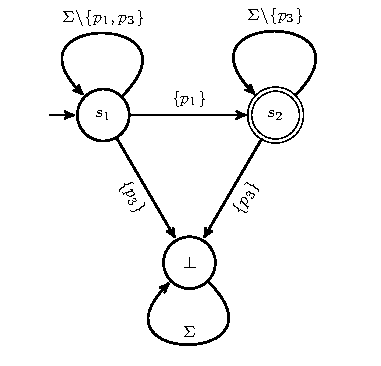
\includegraphics[width=\textwidth]{images/example_1_graph}
%		\caption{$\bot\Release(\neg p_3\vee p_1\vee p_2) \wedge \top\mathcal{U}p_1$}
%		\label{fig:g1}
%	\end{subfigure}
%	\hfill
%	\begin{subfigure}[b]{0.45\textwidth}
%
%	\end{subfigure}
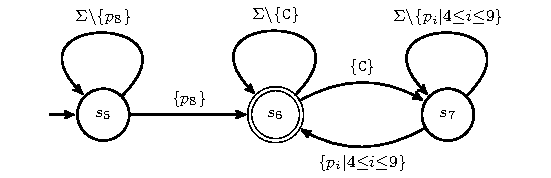
\includegraphics[scale=0.9]{images/example_3_graph}
%\caption{$\bot\Release(\neg\texttt{A}\vee(\top\Until(p_2\vee p_3)))\wedge\top\Until p_3$}
%\label{fig:g2}
	\caption{Representation of the LTL$_f$ formula $\lglobally(\neg\texttt{C}\vee(\lfuture(p_4\vee p_5\vee p_6\vee p_7\vee p_8\vee p_9)))\wedge \lfuture p_8$  as a constraint automaton \cite{Westergaard11}, where $\Sigma$ contains all the non-$\bot$ and non-$\top$ atoms.}
	\label{fig:g1g2}
\end{figure}

\section{Working Assumptions}\label{sec:wa}

In this section, we outline some working assumptions that can be inferred from the literature of reference. First, we assume that \begin{enumerate*}[label=\emph{\alph*})]
\item compliance requirements of Declare models can be expressed in a formal language such as Linear Time Logic on Finite Traces (LTL$_f$) \cite{GiacomoV13}, as business process logs contain only traces of finite length;
\item we restrict the space of the possible alignments of the log trace repairs to the traces generated by the automaton representation of the Declare model;
%\item as in \cite{XuLZ17a}, we want to align a single log trace against a declare model, thus restricting the space of the possible alignments;
\item differently from \cite{MultiPerspective}, we can avoid to model reading and writing operation, as the entirety of our analysis will be conducted once traces \DIFadd{reach their completion}; \item last, each event trace must be represented by one single proposition: similarly to the non-data aware scenario \cite{XuLZ17a}, each event trace should be associated to just one activity label. \end{enumerate*} As we will see in the incoming section, the latter consideration will require us to partition the possible data space into distinct propositions.


%Still, we can freely assume that the constraint automatons generated from the LTL$_f$ interpretation of such Declare constraints allow to represent any possible event label that is not represented within the Declare constraints, by either representing it as a transition $\Sigma\backslash S$, where $\Sigma$ is the set of all the possible strings and $S$ is a (possibly empty) finite set of traces that we want to ignore \cite{LeoniMA12,Westergaard11}, or by representing it as finite conjunction of negated predicates \cite{Lydia}, where each predicate is a proposition that can be deduced from a Declare Model represented in LTL$_f$. Figure~\ref{fig:g1g2} provides a intuitive representation of some LTL$_f$ formulae in the former representation.


Given an appropriately chosen set $\Sigma$ of atoms, it is always possible to represent a trace $\sigma=\sigma_1\cdots \sigma_n$ as a finite sequence $t_\sigma=t_1\cdots t_n$, where, for $1\leq i\leq n$, $t_i$ is a unique atom $t_i\in\Sigma$ such that $\sigma_i\vDash t_i$ \cite{XuLZ17a}.
Contextually,  any LTL$_f$ formula $\varphi_{\mathcal{M}}$ representing a Declare model $\mathcal{M}$ can be represented as a deterministic finite-state automaton (DFA) $\mathcal{A}_{\varphi_{\tiny\mathcal{M}}}$ \cite{Westergaard11} accepting all the sequences $t_\sigma$ from traces $\sigma$ satisfying $\varphi_{\mathcal{M}}$ (see Figure~\ref{fig:g1g2}). A DFA  $(\Sigma,Q,q_0,\rho,F)$ is defined \cite{0016921} over a finite set of states $Q$ reading as input symbols from a finite alphabet $\Sigma$ that are consumed by traversing the automaton from a starting state $q_0\in Q$ via a transition function $\rho\colon Q\times \Sigma\to Q$; the input sequence is accepted once the input sequence is completely digested and an accepting state in $F\subseteq Q$ is reached through navigation. Since in the non data-aware Declare scenario the atoms within LTL$_f$ could be either $\top$, or $\bot$, or $\psi=\texttt{A}$, $\Sigma$ corresponds to the activity set  $\textsf{Act}$, as each event is associated to one single label. For data-aware Declare we will extend $\Sigma$ to take into consideration propositional formulas representing data conditions.

Last, we freely assume that all the events having the same label will always contain the same set of keys, with possibly differently associated values. This is a common assumption in the relational database field, where all the rows belonging to the same table contain the same number of values. We also freely assume that missing values are represented with specific values, such as an empty string, $-1$, or $-\infty$, depending on the type. 
\section{Data-Aware Declarative Conformance Checking as Planning}\label{sec:dccap}
In this section, we study the problem of aligning log traces $\sigma\in\mathcal{L}$ and a (data-aware) Declare model $\mathcal{M}$ for data-aware declarative conformance checking: to do so, we firstly reduce such problem to a mere automaton sequence acceptation task via a specific set of atoms $\Sigma$ (\textit{Cf.} \S\ref{sec:wa}) generated from the compound atoms in $\mathcal{M}$: the finite sequence $t_\sigma$ generated from the log trace $\sigma$ is going to be accepted by the automaton $\mathcal{A}_{\varphi_{\mathcal{M}}}$ iff. $\sigma$ is conformant to the model $\mathcal{M}$ (\S\ref{sec:dadtap}). Next, we are going to code $t_\sigma$ and $\mathcal{A}_{\varphi_{\mathcal{M}}}$ as specific automata (\S\ref{ssec:amfta}) that are going to be exploited by a PDDL planner to generate the minimally repaired sequence $\hat{t_\sigma}$ of $t_\sigma$ (\S\ref{ssec:eip}), out of which we generate the minimally repaired trace $\hat{\sigma}$ which is conformant from $\mathcal{M}$ (\S\ref{ssec:trerepair}).


%%the finite sequence $t_\sigma$ generated from $\sigma$ by replacing the events with the satisfied atoms in $\Sigma$ is going to be accepted by the automaton $\mathcal{A}_{}$


%% a sequence acceptation task over an automaton by generating a specific set of atoms $\Sigma$ out of \dots

%%In this section, we demonstrate that assessing the conformance checking of a log trace $\sigma$ containing payloads against a (data-aware) Declare model $\mathcal{M}$ can be reduced to the sequence acceptation problem in \S\ref{sec:wa} by choosing a specific set of atoms $\Sigma$ partitioning the data space (\S\ref{sec:dadtap}). Then, we can exploit $\Sigma$ to generate a string sequence $t_\sigma$ from $\sigma$ and a DFA for $\mathcal{M}$, from which we will generate two further automata accepting \cite{XuLZ17a,MaggiMCA18} (\S\ref{ssec:amfta}). Last, we can encode such technique as a planning problem in PDDL by adding a novel \texttt{replacement} planning action (\S\ref{ssec:eip}).

%Given a Declare model $\mathcal{M}=\Set{c_i}_{1\leq i\leq m}$, we can always express $\mathcal{M}$ as one single LTL$_f$ formula $\varphi=\bigwedge_{1\leq i\leq m}\varphi_i$, where $\varphi_i$ is the LTL$_f$ translation of the Declare constraint $c_i\in\mathcal{M}$ \cite{LeoniMA12}.
%
%
%
%We can then translate  \cite{0016921} and that LTL$_f$ formulae can be modeled as deterministic finite-state automata (DFAs) \cite{Westergaard11,Lydia}.
%
%Given that Declare semantics can be expressed as LTL$_f$, we can directly analyse such language having the following syntax:
%\[\varphi::=\phi\;|\;\neg \varphi\;|\;\varphi_1\wedge\varphi_2\;|\;\Next \varphi_1\;|\;\varphi_1\Until\varphi_2\]
%where $\phi\in \mathsf{Prop}$, while $\Next$ and $\Until$ are respectively the \textit{next} and \textit{until} operators. This is the functionally complete set of connectives, with which we can express  disjunction ($\vee$),  logical implication ($\Rightarrow$),  equivalence ($\Leftrightarrow$), globally ($\Globally$), finally ($\Finally$), weak until ($\Wntil$), and release ($\Release$) as in \cite{XuLZ17a}. Given a finite trace $\sigma=\sigma_1\cdots \sigma_n$ of length $|\sigma|=n$, the satisfiability of $\varphi$ over the $i$-the event in $1\leq i\leq |\sigma|$, namely $\sigma_i\vDash \varphi$, is inductively defined as follows:
%\begin{itemize}
%	\item $\sigma_i\vDash\phi$ iff. $\sigma_i\vDash\phi$, $\phi\in \mathsf{Prop}$
%	\item $\sigma_i\vDash\neg\varphi$ iff. $\sigma_i\not\vDash\varphi$
%	\item $\sigma_i\vDash\varphi_1\wedge\varphi_2$ iff. jointly $\sigma_i\vDash\varphi_1$ and $\sigma_i\vDash\varphi_2$
%	\item $\sigma_i\vDash\Next\varphi$ iff. $\sigma_{i+1}\vDash\varphi$ with $1\leq i< |\sigma|$
%	\item $\sigma_i\vDash\varphi_1\Until\varphi_2$ iff. it exists $i\leq j\leq |\sigma|$ such that $\sigma_j\vDash\varphi_2$ and, for each $i\leq k<j$, $\sigma_k\vDash\varphi_1$
%\end{itemize}
%Given the working assumptions in \S\ref{sec:wa} and the interpretation of the Declare templates in LTL$_f$, we can restrict $\phi$ to a propositional formulas containing either the universal truth or falsehoods, or predicates $\psi(\sigma_i)$ in the form $\texttt{A}(\sigma_i)\wedge \phi^d(\sigma_i)$.  We say that $\sigma$ satisfies $\varphi$, namely $\sigma\vDash\varphi$, if $\sigma_1\vDash\varphi$. Given that any  Declare clause can be expressed in terms of LTL$_f$ \cite{10.1007/978-3-642-40176-3_8}, any possible  Declare model can be expressed as the conjunction of the LTL$_f$ representations of the  Declare clauses within the model.
%
%\cite{XuLZ17a} showed that we can reduce the conformance checking strategy into a trace alignment problem by following those subsequent steps.
%
%Firstly,  $\sigma\vDash\varphi$ can be proved by
% \begin{enumerate*}[label=\emph{\alph*})]
%\item  picking an alphabet $\Sigma$,
%\item  picking a transformation $\tau$ of traces $\sigma$ into strings $\tau(\sigma_1\cdots \sigma_n)=\tau(\sigma_1)\cdots \tau(\sigma_n)=t_1\cdots t_n$ in $\Sigma^*$,
%\item  picking a bijection $p_i\xleftrightarrow{f}\psi_i$ between $p_i\in\Sigma$ and atoms $\psi_i$ in $\varphi$, and
%\item  transforming $\varphi$ into a  DFA\footnote{}  $\mathcal{A}$
%\end{enumerate*} %and a bijection $p_i\xleftrightarrow{f}\psi_i$ and $\varphi$ into a finite-state automaton
%such that $t_1\cdots t_n$ is accepted by $\mathcal{A}$ iff. %$\sigma\vDash\varphi$. This happens when
%, for $1\leq i\leq |\sigma|$, it always exists a transition $q_i\xrightarrow{p_i}q_{i+1}$ in $\mathcal{A}$ for which $\psi_i(\sigma_i)$ and, for $i=|\sigma|$, $q_{|\sigma|+1}$ is also an accepting state for $\mathcal{A}$. In the non data-aware  scenario where the set of all the possible activity labels $\textsf{Act}$ is finite and atoms $\psi_i$ are always in the form of $\texttt{A}$ with $\texttt{A}\in\textsf{Act}$ \cite{XuLZ17a,Westergaard11}, this reduces to choose
% \begin{enumerate*}[label=\emph{\alph*})]
%	\item  $\textsf{Act}$ as $\Sigma$,
%	\item  $\lambda$ as the transformation $\tau$,
%	\item  use the immediate bijection $\texttt{A}\xleftrightarrow{f}\texttt{A}$, and
%	\item  to generate a DFA from the automata in Figure~\ref{fig:g1g2} from $\varphi$ by replacing an edge $q_i\xrightarrow{S}q_j$ with $q_i\xrightarrow{\texttt{A}}q_j$ for each $\texttt{A}\in S$.
%\end{enumerate*} On the other hand, we can observe that the representation of $\psi_i$ as a combination of atoms is less straightforward in a general data-aware Declare scenario, as we must guarantee that each event $\sigma_i$ is transformed into one single symbol in $\Sigma$ (see also \S\ref{sec:wa}). For this reason, we firstly show how we can build such set of atoms $\Sigma$:
%

%\begin{lemma}
%It always possible to decompose a proposition $\psi(\sigma_i)=\texttt{A}(\sigma_i)\wedge \phi^d(\sigma_i)$ from an LTL$_f$ interpretation of a Declare model $\mathcal{M}$ via a disjunction of atoms in $\Sigma$ such that each event $\sigma_i$ satisfies only one atom in $\Sigma$.
%\end{lemma}
%\begin{proof}
%Figure~\ref{fig:twoexamples} provides an intuitive sketch of the proof. In more detail, after representing each constraint $c_i\in\mathcal{M}$ (step 1) as an LTL$_f$ formula (step 2) in \textit{negated normal form} (\textit{nnf}), we colle
%\end{proof}
%
%%Secondly, we can transform the constraint automaton $\mathcal{A}$ into an augmented automaton $\mathcal{A}$ accepting all the traces satisfying $\varphi$
%%%
%%\begin{proof}	
%%Given that non-deterministic finite-state automata (NFA) accept the same language of deterministic finite-state automata \cite{0016921} and that LTL$_f$ formulae can be modeled as DFAs \cite{Westergaard11,Lydia}, there exists a transformation for  $\varphi$ into a deterministic finite-state automaton $\mathcal{A}$ (\textit{constraint automaton}) and one for $\sigma$ into a deterministic finite-state automaton $\mathcal{T}$ (\textit{trace automaton}) as a single (accepting) path such that, if $\mathcal{T}$ is (also) an accepting path for $\mathcal{A}$, then $\sigma\vDash\varphi$ \cite{XuLZ17a}.
%%\end{proof}
%%
%%
%%
%%We can show that the declarative conformance checking can be modeled as a trace alignment problem by firstly transforming a Declare model as a deterministic finite-state automaton (DFA) via an LTL$_f$ formula, namely \textit{constraint automaton} $\mathcal{A}$, as well as directly translating the trace $\sigma$ as another DFA, namely \textit{trace automaton} $\mathcal{T}$, which is formed by one single path accepting $\sigma$. Last, we need to show that $\mathcal{A}$ contains the exact path $\mathcal{T}$
%%
%%We can represent $\sigma$ as a DFA $\mathcal{T}=(\Sigma_\sigma,Q_\sigma,q_0^\sigma,\rho_\sigma,F_\sigma)$, namely a \textit{trace automaton} \cite{XuLZ17a}, having having \begin{enumerate*}[label=\emph{\alph*})]
%%	\item $\Sigma_\sigma=\Set{\sigma_1,\dots,\sigma_n}$,
%%	\item $Q_\sigma=\Set{q_0^\sigma,\dots,q_n^\sigma}$ a set of arbitrary $|\sigma|+1$ states, with
%%	\item an initial state $q_0^\sigma$ and
%%	\item a set $F=\Set{q_n^\sigma}$ of accepting states, where
%%	\item the transition relation $\rho_\sigma(q_i^\sigma,\sigma_i)=q_{i+1}^\sigma$ for each $1\leq i\leq |\sigma|+1$.
%%\end{enumerate*}
%%Every LTL$_f$ formula can be directly associated to a deterministic finite-state automaton (DFA) $\mathcal{A}=(\Sigma,Q,q_0,\rho,F)$, namely a \textit{constraint automaton}, accepting only the traces satisfying $\varphi$ \cite{Lydia}, having \begin{enumerate*}[label=\emph{\alph*})]
%%	\item an input alphabet $\Sigma\subseteq \textsf{Prop}$,
%%	\item a finite set $Q$ of states, with
%%	\item an initial state $q_0\in Q$ and
%%	\item a set $F\subseteq Q$ of accepting states, where
%%	\item the latter can be reached from the former via a transition relation $\rho\colon Q\times \Sigma\to Q$.
%%\end{enumerate*} Furthermore,
%%
%%\[s_{\mathcal{A},\sigma}(q,i)=\begin{cases}
%% 	\textbf{true} & i>|\sigma|\wedge q\in F\\
%% 	s_{\mathcal{A},\sigma}(q,i+1) & i\leq |\sigma|\wedge \exists! \phi. \rho(q,\phi)
%%\end{cases}\]
%%
%%\bigskip
%
%Secondly, the authors introduced \textit{repair atoms}  \texttt{del\_a} (or \texttt{add\_a}) for each $\texttt{A}\in\Sigma$ respectively remarking that \texttt{A} was removed (or added) in the input trace, while it needs to be added (removed) to make the string accepted. This allows to transform $\mathcal{A}$ into $\mathcal{A}^+$ accepting all the repaired strings $\tilde{t}$ from $t$ \texttt{\color{red}[TODO]}
%
%





\subsection{$\Sigma$-encoding for conformance checking}\label{sec:dadtap}
As per the previous considerations, we want to show that to solve the trace alignment problem for data-aware declarative conformance checking, it is sufficient to provide a specific characterization of $\Sigma$. $\Sigma$ will be used to generate an automaton accepting symbols in $\Sigma$ and the automaton will be used to test log traces represented as finite sequences in $\Sigma^*$. The proposed approach for obtaining $\Sigma$ from a (data-aware) Declare model $\varphi_{\mathcal{M}}$ is sketched in Figure~\ref{fig:twoexamples}, and described in detail in the following.

\begin{table*}[!t]
	\centering
	\captionsetup[subtable]{position = below}
	\captionsetup[table]{position=top}
	\caption{Intermediate steps for generating distinct atoms for \texttt{B} labelled events by partitioning the data space via intervals in Declare clauses.}
	\begin{subtable}{0.45\linewidth}
		\centering
		\resizebox{\textwidth}{!}{%
						\begin{tabular}{c|c||c|c|}
				\toprule
				\multicolumn{2}{c||}{$\mu(\texttt{B},x)$} & \multicolumn{2}{c}{$\mu(\texttt{B},y)$}\\
				\midrule
				$\texttt{B}.x>3$      & $\texttt{B}.x>3$ & $\texttt{B}.y=0$ & $0\leq \texttt{B}.y\leq 0$\\
				$\texttt{B}.x> 0$ & $0<\texttt{B}.x\leq 3$, $ \texttt{B}.x>3$ & $\texttt{B}.y\neq 0$ & $\texttt{B}.y<0\vee \texttt{B}.y>0$\\
				$\texttt{B}.x\leq 0$ & $ \texttt{B}.x\leq 0$ & & \\
				\bottomrule
			\end{tabular}%
		}
		\caption{Interval decomposition in $\mu(\cdot, \cdot)$}
		\label{tab:dimFFT}
	\end{subtable}\quad
	\begin{subtable}{0.6\linewidth}
		\centering
		\resizebox{.5\textwidth}{!}{%
			\begin{tabular}{c|ccc}
	\toprule
	\texttt{B} & $\texttt{B}.y< 0$ & $\texttt{B}.y=0$ & $\texttt{B}.y>0$ \\
	\midrule
	$\texttt{B}.x\leq 0$ & $p_1$ & $p_2$ & $p_3$   \\
	$0<\texttt{B}.x\leq 3$ & $p_4$ & $p_5$ & $p_6$\\
	$\texttt{B}.x>3$ & $p_7$ & $p_8$& $p_9$ \\
	\bottomrule
\end{tabular}%
		}
		\caption{Atom generations for \texttt{B} by data space partitioning via $\times_{k\in K}\mu(\texttt{B},k)$}
		\label{tab:dimGMM}
	\end{subtable}
\end{table*}

\begin{figure}[!t]
	\centering
	%{\hspace{-1.3cm}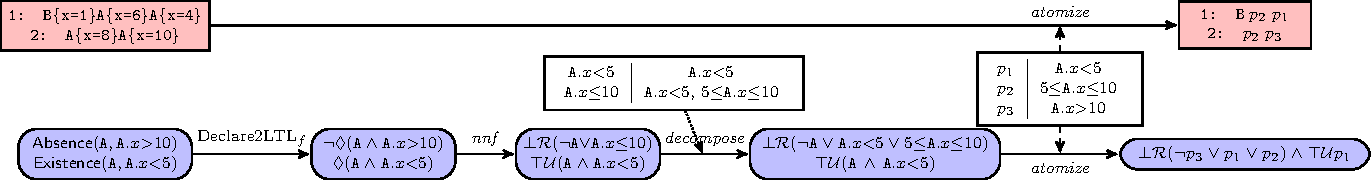
\includegraphics[width=1.3\textwidth]{images/example_1}}
	{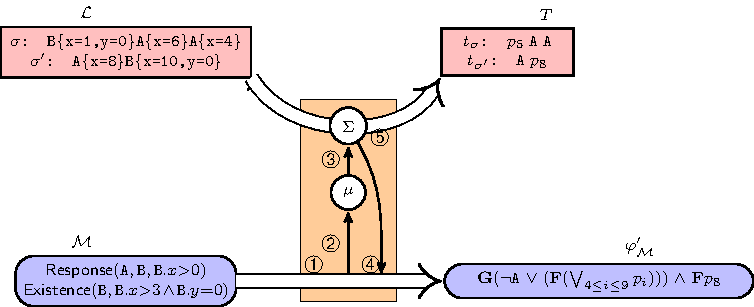
\includegraphics[width=.7\textwidth]{images/example_3}}
	\caption{Intermediate steps required for obtaining $\Sigma=\Set{p_i|1\leq i\leq 9}\cup\{\texttt{C}\}$ from $\mathcal{M}$ and transforming $\mathcal{L}=\Set{\sigma,\sigma'}$ to a set of finite sequences $T=\Set{t_\sigma,t_{\sigma'}}$, as well as replacing atoms in $\varphi_{\mathcal{M}}$ with equivalent atoms in $\Sigma$ ($\varphi_{\mathcal{M}}'$).}\label{fig:twoexamples}
\end{figure}

In the first \emph{Declare2LTL}$_f$ step, we exploit the usual conversion of each single Declare clause into an LTL$_f$ formula (see Table 1) in the \textit{negated normal form} \cite{LiPZVR20}, where negations are possibly pushed inside atoms ``$\texttt{A}.k\;\Re\; c$'' by replacing $\Re$ with its negation.
\begin{ex} \label{ex:first}
The Declare model $\mathcal{M}$ containing the  clauses $\mathsf{Response}(\texttt{C},\texttt{B},\;\texttt{B}.x>0)$ and
$\mathsf{Existence}(\texttt{B},\; \texttt{B}.x>3\wedge \texttt{B}.y=0)$ is represented as the intermediate LTL$_f$ formula $\varphi_{\mathcal{M}}=\lglobally(\neg\texttt{C}\vee \lfuture(\texttt{B}\wedge \texttt{B}.x>0))\wedge \lfuture(\texttt{B}\wedge \texttt{B}.x>3\wedge \texttt{B}.y=0)$.
\end{ex}




In the second \textit{decomposition} step, for each compound condition $\psi=\texttt{A}\wedge \phi^d$ over labels $\texttt{A}\in\textsf{Act}$, we collect all the atoms in $\phi_d$ in the form ``$\texttt{A}.k\;\Re\; c$'' for each $k\in K$ in a map $\mu(\texttt{A},k)$. Contextually, we represent each atom as an interval, and we \textit{decompose} them
%
%%We now describe the main contribution of the paper, namely a technique for computing log trace alignments over Declare data-aware models. Our approach takes as input \begin{enumerate*}[label=\emph{\alph*})]
%	\item a Declare data-aware model $\mathcal{M}$ expressed as a set of instantiated templates,
%	\item a log trace $\sigma$,
%\end{enumerate*} and ranks the outcome of a LTL$_f$ conformance checking $\sigma\tilde{\vDash}\varphi$ accordingly to a data distance function $\mathcal{D}$.
%
%%The input transformation for reducing the data-aware alignment problem to the data-agnostic one is presented in Figure~\ref{fig:twoexamples} for two alignment examples. In particular, we first transform the data-aware Declare model, for then collecting the required information for providing the trace transformation.
%
%%\textbf{data-aware Declare Model Processing.}
%
%
%
%
%%In step 3, we collect the data-aware predicates ``$\texttt{A}.\textit{var}\;\Re\;c$'' from all the model's clauses and group them by $\texttt{A}.\textit{var}$; each of these predicates is \textit{decomposed}
into a disjunction of maximal non-overlapping data-aware predicates. This task can be efficiently computed via interval trees \cite{inttree}. Last, we replace the atoms in each LTL$_f$ formula by its decomposed representation.%, if any.
\begin{continueexample}{ex:first}\label{ex:second}
Table~\ref{tab:dimFFT} shows the interval decomposition results for the $\psi$ extracted from $\mathcal{M}$. E.g., predicates $\texttt{B}.x>3$ and $\texttt{B}.x>0$ are first represented as intervals $\interval({3,+\infty})$ and $\interval({0,+\infty})$, and then decomposed into disjoint sub-intervals $\interval({-\infty,0}]$, $\interval({0,3}]$, and $\interval({3,+\infty})$. As a result, $\varphi_{\mathcal{M}}$ is decomposed into $\varphi_{\mathcal{M}}^d=\lglobally(\neg\texttt{C}\vee \lfuture(\texttt{B}\wedge \texttt{B}.x>0))\wedge \lfuture(\texttt{B}\wedge (0<\texttt{B}.x\leq 3\vee \texttt{B}.x> 3) \wedge \texttt{B}.y=0)$
\end{continueexample}

In the third \textit{atomization} step, we put an atom $\texttt{A}\in\textsf{Act}$ in $\Sigma$ if the map $\mu(\texttt{A},k)$ is empty for each key $k\in K$; otherwise, given all the keys $k_{\texttt{A}_1},\dots,k_{\texttt{A}_h}\in K$ for which the map $\mu(\texttt{A},k_{\texttt{A}_i})$ is not empty, we partition the data space by combining the non-overlapping intervals as $\mu(\texttt{A},k_{\texttt{A}_1})\times\cdots\times\mu(\texttt{A},k_{\texttt{A}_h})$ obtained from the previous step. For each of these interval combinations, we generate a fresh atom and put it in $\Sigma$.
\begin{continueexample}{ex:first}
Label \texttt{C} is never associated to a data condition, and therefore it will be associated to one single atom \texttt{C}. On the other hand, label \texttt{B} is associated to several atoms obtained by partitioning the data space via the intervals in Table~\ref{tab:dimFFT}. Table~\ref{tab:dimGMM} shows the atom decomposition of \texttt{B} via data intervals over keys $x$ and $y$, which induce a space partitioning of 9 intervals, for which we generate nine distinct atoms $p_1\dots p_9$. As a result, we obtain $\Sigma=\Set{p_i|1\leq i\leq 9}\cup\Set{\texttt{C}}$ in Figure~\ref{fig:twoexamples}.
\end{continueexample}


%In step 4, for each event label \texttt{C}, we partition the data space \textit{var}$_1\times\dots\times$\textit{var}$_h$ associated to \texttt{C} by exploiting the disjoint intervals mined in the previous step. Each of such combination will be syntactically represented as a fresh \textit{atom}  proposition $p_i$: this implies that the label \texttt{C} is represented by the disjunction $\bigvee_ip_i$. When the data space associated to the predicates mined for \texttt{C} has only one property,  the atoms corresponds to the ones mined in the previous step. E.g., \texttt{C} in the first example from \ref{fig:twoexamples} is equivalent to $p_1\vee p_2\vee p_3$, and $\texttt{C}.\textit{x}<5$ is rewritten as $p_1$; given that such atoms represent disjoint intervals, then $\texttt{C}\wedge p_1\equiv p_1$. Similarly, $\neg \texttt{C}\vee \texttt{C}.\textit{x}<5\vee 5\leq\texttt{C}.\textit{x}\leq 10$ can be immediately rewritten as $\neg(p_1\vee p_2\vee p_3)\vee p_1\vee p_2$, which is equivalent to $\neg p_3\vee p_1\vee p_2$. Last, each LTL$_f$ representation of a data-aware Declare clause is represented into one si\ding{193}ngle LTL$_f$ formula by conjunction and simplification.


Starting from these atoms, we firstly replace the compound conditions in the LTL$_f$ interpretation $\varphi_{\mathcal{M}}$ of $\mathcal{M}$ with a disjunction of atoms from $\Sigma$ as described in Table~\ref{tab:dimGMM}, thus obtaining an equivalent LTL$_f$ formula $\varphi_{\mathcal{M}}'$. Secondly, we generate a finite sequence $t_\sigma\in T$ for each log trace $\sigma\in\mathcal{L}$ by replacing each event $\sigma_i$ in $\sigma$ with the only atom $t_i\in \Sigma$ such that $\sigma_i\vDash t_i$.
%
%\textbf{data-aware Log Trace Processing.} Given the atomization in Step 4, we process each data-enriched event within the trace as follows: if the event label is never associated with a data predicate, then we just discard the data information; otherwise, we replace each event with the single corresponding atom satisfying the associated semantics. Please observe that, by previous construction, each event can be represented by just one possible propositional atom, as the previous construction guarantees a partitioning (thus non-overlapping) representation of the data space.

\begin{continueexample}{ex:first}
With reference to our running example, we replace the compound conditions in $\varphi_{\mathcal{M}}^d$ with the previously generated atoms; the compound condition $\texttt{B}\wedge \texttt{B}.x>0$ is replaced by all the possible configurations of $y$ and data intervals $0<\texttt{B}.x\leq 3$ and $\texttt{B}.x>3$, which are identified by the disjunction $p_4\vee p_5\vee p_6\vee p_7\vee p_8\vee p_9$. On the other hand, $\texttt{B}\wedge\texttt{B}.x>3\wedge \texttt{B}.y=0$ can be directly replaced by atom $p_8$: this results into an equivalent formula $\varphi_{\mathcal{M}}'=\lglobally(\neg\texttt{C}\vee(\lfuture(p_4\vee p_5\vee p_6\vee p_7\vee p_8\vee p_9)))\wedge \lfuture p_8$.
Given a log $\mathcal{L}=\{\texttt{B\{x=1,y=0\}C\{x=6\}C\{x=4\}},
\texttt{ C\{x=8\}B\{x=10,y=0\}}\}$,
all the events labeled as \texttt{C} are replaced with the atom \texttt{C}, as there are no (data) conditions in $\mathcal{M}$ that we can exploit to partition the data space. On the other hand, each event labeled as \texttt{B} is replaced by an equivalent atom in $\Sigma$: event \texttt{B\{x=1,y=0\}} is uniquely represented by $p_5$, while event \texttt{B\{x=10,y=0\}} is uniquely represented by $p_8$. %Similar considerations can be drawed for the $\psi$ compound atoms in $\varphi_{\mathcal{M}}$ where compound conditions are replaced into an equivalent disjunction of atoms in $\Sigma$:
This transformation results into a set of string sequences $T=\{{ p_5\;\texttt{C\;C}}, \texttt{ C}\;p_8\}$.

\end{continueexample}


After generating $\varphi_{\mathcal{M}}'$, we can exploit existing approaches \cite{Westergaard11} to generate a DFA that only accepts sequences satisfying $\varphi_{\mathcal{M}}'$. With reference to the previous example, the first trace is not conformant with $\mathcal{M}$, since the first sequence is not accepted by the associated automaton. Similarly, the second trace is conformant with $\mathcal{M}$, since the second sequence is accepted by the associated DFA. In the forthcoming subsection, we will discuss how to generate repaired sequences that are accepted by the reference model.

\subsection{Automaton Manipulation for Trace Alignment}\label{ssec:amfta}
Consider a sequence $t_\sigma=t_1\cdots t_n$ generated from a trace $\sigma$, and the constraint automaton $\mathcal{A}_{\varphi_{\mathcal{M}}}$ generated from the Declare model $\mathcal{M}$, both generated via a set of atoms $\Sigma$. If the trace is deviant with respect to the model, we are interested in generating a repair sequence $\varrho=\varrho_1\cdots \varrho_m$ from $t_\sigma$ describing the operations to perform over $\sigma$ to make it conformant to the model $\mathcal{M}$.

To realize this transformation, we consider two types of atomic violations, which can be caused by wrong (\textit{deletion}) or missing (\textit{insertion}) atoms in $\Sigma$. Differently from the non-data aware case, here, we also need to model \textit{replacement} operations, defined as a data update within one single trace event: these operations can be mimicked by a delete operation followed by an insertion, as they substitute an event within a trace with the same event where a data value has been updated. The above operations can be defined as follows:
\begin{itemize}
	%\item synchronization $[\sigma_k\leftrightarrow \phi]$ aborts if $\sigma_k\neq\phi$, for  $1\leq k\leq |\sigma|$
	\item \textit{deletion}\,\, $[\#\sigma_k\leftarrow \phi]::= \sigma_1\cdots\sigma_{k-1}\sigma_{k+1}\cdots \sigma_n$,\,\,\, for $n=|\sigma|$, $1\leq k\leq n$, and $\phi=\sigma_k$
	\item \textit{insertion} $[@\sigma_k\leftarrow \phi]::= \sigma_1\cdots\sigma_{k-1}\phi\sigma_{k}\cdots \sigma_n$,\,\,\,\,\,\,\,\,\,\,\,\, for $n=|\sigma|$ and $1\leq k\leq n$
	\item \textit{replacement} $[\sigma_k[\phi\mapsto\phi']]::=\sigma_1\cdots \sigma_{k-1}\phi'\sigma_{k+1}\cdots\sigma_n$ for $n=|\sigma|$, $1\leq k\leq n$, and $\phi=\sigma_k$
\end{itemize}
Each of these operations has an associated cost, either quantifying the severity of the found violation or determining which operations shall be preferred. E.g., by assigning a higher cost to insertions and deletions and a lower one to replacements, we will favor replacements when possible. The \textit{alignment cost} is defined as the number of deletions multiplied by their cost, plus the number of insertions multiplied by their cost, plus the number of replacements multiplied by their cost.

We can now define the conformance checking problem as follows:
\begin{definition}[Log/Declare Conformance Checking]
Given a trace $\sigma$ and a Declare model $\mathcal{M}$, either $\sigma$ conforms to $\mathcal{M}$, or $\sigma$ is deviant and it exists a repair sequence $\varrho$ both making $\sigma$ non-deviant for $\mathcal{M}$ and guaranteeing a minimal transformation cost.
\end{definition}

%\texttt{\color{red}[TODO]} we consider insertions and deletions as possible repairs, while substitutions can be modeled by deletions followed by insertions. Synchronizations are \texttt{noops} requiring that a trace $\sigma$ at step $k$ contains a predicate $\phi$.
%%
%Therefore, any repair  of a trace $\sigma$ can be expressed in terms of a sequence of operations $\texttt{op}_1\cdots \texttt{op}_m$ which, when executed in appearance order, generate a novel trace $\tilde{\sigma}$ from $\sigma$.  \texttt{\color{red}[TODO]}
%%
%
%Last, the amount of repairs can be numerically quantified using a cost function $\mathcal{C}$ returning zero for any synchronization and $1$ otherwise; therefore $cost(\sigma, \tilde{\sigma})$ returns the minimal number of non-synchronization operations\footnote{Formally, $cost(\sigma,\tilde{\sigma})=\min_{\substack{\texttt{op}_1\cdots \texttt{op}_m,\\(\texttt{op}_m\,\circ \cdots\circ\, \texttt{op}_1)(\sigma)=\tilde{\sigma}}}\sum_{1\leq i\leq m}\mathcal{C}(\texttt{op}_m)$} required to obtain $\tilde{\sigma}$ from $\sigma$. Therefore, the conformance checking of a log trace $\sigma$ against a  Declare model represented as an LTL$_f$ formula $\varphi$ as in \cite{XuLZ17a} either returns $\sigma$ with cost zero if $\varphi\vDash\varsigma$ or, otherwise, returns a set of pairs $\Set{\braket{\tilde{\sigma},\texttt{op}_1\cdots\texttt{op}_m}_i}_{1\leq i\leq k, k\in\mathbb{N}}$, where\footnote{Formally, $\sigma\tilde{\vDash}\varphi = \Set{\braket{\tilde{\sigma},\texttt{op}_1\cdots\texttt{op}_m} | cost(\sigma,\tilde{\sigma}) = \min_\mu cost(\sigma,\mu),\;\tilde{\sigma}\vDash\varphi,\; (\texttt{op}_m\,\circ \cdots\circ\, \texttt{op}_1)(\sigma)=\tilde{\sigma}}$.} each trace $\tilde{\sigma}\in S$ is conformant to $\varphi$ and minimizes the alignment cost $cost(\sigma,\tilde{\sigma})$ via a repair sequence $\texttt{op}_1\cdots\texttt{op}_m$. We denote the output of such conformance checking as $\sigma\tilde{\vDash}\varphi$.

The process of generating a repair sequence can be addressed by resorting to DFAs (\S\ref{sec:wa}). Let $t_\sigma=t_1\cdots t_n$ be a string sequence generated from a log trace $\sigma$ via $\Sigma$, $\mathcal{A}_{\varphi_{\mathcal{M}}}=(\Sigma,Q,q_0,\rho,F)$ the constraint automaton to check $t_\sigma$ against. From $t_\sigma$, we define a further automaton, called the \textit{trace automaton} $\mathcal{T}=(\Sigma_t,Q_t,q_0^t,\rho_t,F_t)$ having \begin{enumerate*}[label=\emph{\alph*})]
	\item $\Sigma_t=\Set{t_i|t_i\in t_\sigma}$,
	\item $Q_t=\Set{q_0^t,\cdots,q_n^t}$ as a set of $|t_\sigma|+1$ states,
	\item $\rho(q_i^t,e_{i+1})=q_{i+1}^t$ for $0\leq i\leq n-1$,
	and
	\item $F_t={q_n^t}$.
\end{enumerate*} By definition, such a graph accepts only $t_\sigma$.

\begin{figure}[!t]
	\centering
	{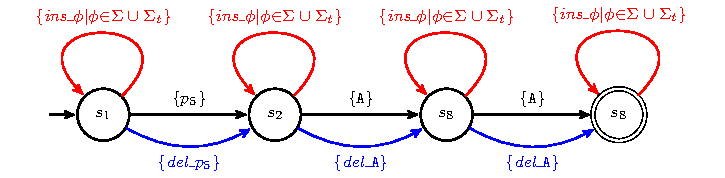
\includegraphics[width=.7\textwidth]{images/Tplus}}
	\caption{Augmented trace automaton $\mathcal{T}^+$ for $t_{\sigma'}=p_5\;\texttt{C}\;\texttt{C}$.}\label{fig:tplus}
\end{figure} \begin{figure}[!t]
\centering
{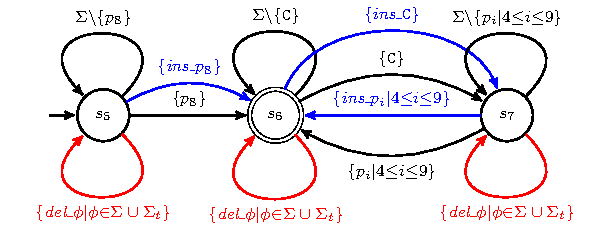
\includegraphics[width=.7\textwidth]{images/Aplus}}
\caption{Augmented constraint automaton $\mathcal{A}_{\varphi_{\mathcal{M}}}^+$ for $\mathcal{A}_{\varphi_{\mathcal{M}}}$.}\label{fig:aplus}
\end{figure}
Next, we augment $\mathcal{T}$ and $\mathcal{A}_{\varphi_{\mathcal{M}}}$ by adding transitions related to just the atomic operations of insertions and deletions: Thus, from $\mathcal{T}$ we generate the automaton $\mathcal{T}^+=(\Sigma_t^+,Q_t,q_0^t,\rho_t^+,F_t)$ having:
\begin{itemize}
	\item $\Sigma_t^+$ extending $\Sigma_t\subseteq \Sigma$ by adding an insertion $\textit{ins\_}\phi$ for each atom $\phi\in\Sigma_t\cup\Sigma$ and a deletion $\textit{del\_}\phi$ for each atom  $\phi\in\Sigma_t$.
	\item $\rho_t^+$ extending $\rho_t$ by adding deletions $\rho_t^+(p,\textit{del\_}\phi)=q$ for each transition $\rho_t(p,\phi)=q$; and, for all atoms $\phi\in\Sigma\cup\Sigma_t$ and states $q\in Q_t$, we add insertions $\rho_t^+(q,\textit{ins\_}\phi)=q$.
\end{itemize}
Figure~\ref{fig:tplus} shows the trace automaton generated from the deviant trace $\sigma_1$ from Example \ref{ex:first}. Similarly, from $\mathcal{A}_{\varphi_{\mathcal{M}}}$, we obtain $\mathcal{A}_{\varphi_{\mathcal{M}}}^+=(\Sigma^+,Q,q_0,\rho^+,F)$ having:
\begin{itemize}
	\item $\Sigma^+$ extending $\Sigma$ by adding an insertion $\textit{ins\_}\phi$ for each atom $\phi\in\Sigma$ and a deletion $\textit{del\_}\phi$ for each atom  $\phi\in\Sigma\cup\Sigma_t$.
\item $\rho^+$ extending $\rho_t$ by adding insertions $\rho^+(p,\textit{ins\_}\phi)=q$ for each transition $\rho(p,\phi)=q$; and, for all atoms $\phi\in\Sigma\cup\Sigma_t$ and states $q\in Q$, we add deletions $\rho_t^+(q,\textit{del\_}\phi)=q$.
\end{itemize}
Figure~\ref{fig:aplus} shows the automaton augmented with the repair operations $\mathcal{A}_{\varphi_{\mathcal{M}}}^+$ obtained for the model $\mathcal{M}$ from Example \ref{ex:first}. Intuitively, $\mathcal{A}_{\varphi_{\mathcal{M}}}^+$ accepts all the string sequences conformant to the model and have been obtained by adding/removing the missing/wrong atoms to/from $t_\sigma$, where atomic operations are explicitly marked. As required, both augmented automata do not accept $t_{\sigma'}=p_5\;\texttt{C}\;\texttt{C}$. However, if we repair the sequence by adding $p_8$ at the end and explicitly remarking such repair operation with $\textit{ins\_}p_8$, we can see that the augmented automata accept $\hat{t_{\sigma'}}=p_5\;\texttt{C}\;\texttt{C}\;\textit{ins\_}p_8$.

Next, we show how automated planners can efficiently identify the repair operations $\varrho$ needed to repair the trace $\sigma$ using the augmented automata just defined.

\subsection{Encoding in PDDL}\label{ssec:eip}

\newcommand{\myi}{\emph{(i)}\xspace}
\newcommand{\myii}{\emph{(ii)}\xspace}
\newcommand{\myiii}{\emph{(iii)}\xspace}
\newcommand{\myiv}{\emph{(iv)}\xspace}
\newcommand{\myv}{\emph{(v)}\xspace}
\newcommand{\myvi}{\emph{(vi)}\xspace}
\newcommand{\A}{\mathcal{A}}
\newcommand{\T}{\mathcal{T}}
\newcommand{\PDDL}[1]{\begin{footnotesize}\texttt{#1}\end{footnotesize}}
%E.g., the alignment result $\hat{t_\sigma}=p_5\;\texttt{A}\;\texttt{A}\;\textit{ins\_}p_8$ of trace $\sigma=$\texttt{B\{x=1,y=0\}A\{x=6\}\\A\{x=4\}} generates the repair $\varrho=[@\sigma_4\leftarrow p_8]$ after removing the \texttt{sync} operations.

\sloppypar

In this section, we show how, given an augmented constraint automaton $\mathcal{A}_{\varphi_{\mathcal{M}}}^+$ obtained from an LTL$_f$ formula  $\varphi_{\mathcal{M}}$, and an augmented trace automaton $\T^+$ obtained from a trace $t$, we build a cost-optimal planning domain $\mathcal{P_D}$ and a problem instance $\mathcal{P}$ in PDDL. $\mathcal{P_D}$ and $\mathcal{P}$ can be used to feed any state-of-the-art planners accepting PDDL 2.1 specifications, as discussed in Section \ref{ssec:ap}.
%
A solution plan for $\mathcal{P}$ amounts to the set of interventions of minimal cost to repair the trace with respect to $\varphi_{\mathcal{M}}'$.

%\paragraph{Planning Domain}
\medskip
\noindent
\textbf{Planning Domain.}
%
In $\mathcal{P_D}$, we provide two abstract types: \PDDL{activity} and \PDDL{state}.
%
The first captures the activities involved in a transition between two different states of a constraint/trace automaton.
%
The second is used to uniquely identify the states of the constraint automaton (through the sub-type \texttt{automaton\_state}) and of the trace automaton (through the sub-type \texttt{trace\_state}).
%
To capture the structure of the automaton and to monitor its evolution, we defined five \emph{domain propositions} as boolean predicates in $\mathcal{P_D}$:
%
\begin{itemize}
	\item \PDDL{(trace ?t1 - trace\_state ?e - activity ?t2 - trace\_state)} holds if there exists a transition in the trace automaton between two states \texttt{t1} and \texttt{t2}, being \texttt{e} the activity involved in the transition.
	\item \PDDL{(automaton ?s1 - automaton\_state ?e - activity ?s2 - automaton\_state)} holds if there exists a transition between two states \texttt{s1} to \texttt{s2} of a constraint automaton, being \texttt{e} the activity involved in the transition.
    \item \PDDL{(atoms ?e1 - activity ?e2 - activity)} holds if \texttt{e1} and \texttt{e2} are two atoms in $\Sigma$ associated to a same activity label.
	\item \PDDL{(cur\_state ?s - state)} holds if \texttt{s} is the current state of a constraint/trace automaton.
	\item \PDDL{(final\_state ?s - state)} holds if \texttt{s} is a final state of a constraint/trace automaton.
\end{itemize}
It is worth to notice that, if a generic activity \texttt{A} is associated to some data condition, \texttt{A} will be represented as a set of atoms $p_1$, $p_2$, $p_3$, etc. in $\mathcal{P_D}$, see for example Table \ref{tab:dimGMM}. This means that, for any combination of atoms $p_i$ - $p_j$ associated to \texttt{A}, there will exist an instance of the predicate \PDDL{(atoms)} that will hold for $p_i$ and $p_j$.
%
%Label \texttt{C} is never associated to a data condition, and therefore it will be associated to one single atom \texttt{C}. On the other hand, label \texttt{B} is associated to several atoms obtained by partitioning the data space via the intervals
%
Furthermore, we define a \emph{numeric fluent} \PDDL{total-cost} to keep track of the cost of the violations. Notice that: \myi in PDDL, parameters are written with a question mark character `?' in front, and the dash character `-' is used to assign types to parameters; and \myii we remain consistent with the PDDL syntax, which allows the values of both predicates and fluents to change as a result of the execution of an action.
%

Planning actions are used to express the \emph{repairs} on the original trace $t$. Each action is characterized by its \emph{preconditions} and \emph{effects}, stated in terms of the domain propositions. In our encoding, we have defined four actions to perform \emph{synchronous moves} both in the trace/constraint automaton, or to add/remove/replace activities to/from/in the constraint and trace automata. In the following, we suppose that actions \PDDL{ins}, \PDDL{del} and \PDDL{repl} have cost equal to 1. However, their cost can be customized to define the severity of a violation or to force priorities among actions.
%
%\begin{tiny}
%	\begin{verbatim}	
%	(:action sync                                          (:action add                              (:action del
%	:parameters (?t1 - path_state                           :parameters (?e - activity)               :parameters (?t1 - path_state
 %                ?e - activity                              :effect (and (increase (total-cost) 1)                  ?e - activity
  %               ?t2 - path_state)                           (forall (?s1 ?s2 - automaton_state)                    ?t2 - path_state)
%	:precondition (and (cur_state ?t1) (path ?t1 ?e ?t2))       (when (and (cur_state ?s1)            :precondition (and (cur_state ?t1)
%	:effect(and (not (cur_state ?t1)) (cur_state ?t2)           (automaton ?s1 ?e ?s2))               :effect(and (increase (total-cost) 1)
%	 (forall (?s1 ?s2 - automaton_state)                        (path ?t1 ?e ?t2))                    (not (cur_state ?t1)) (cur_state ?t2)))
%	   (when (and (cur_state ?s1)                               (and (not (cur_state ?s1))
%	   (automaton ?s1 ?e ?s2))                                  (cur_state ?s2))))))
%	   (and (not (cur_state ?s1))
%	   (cur_state ?s2))))))
%	\end{verbatim}
%\end{tiny}

\begin{scriptsize}
\begin{verbatim}
(:action sync
 :parameters (?t1 - trace_state ?e - activity ?t2 - trace_state)
 :precondition (and (cur_state ?t1) (trace ?t1 ?e ?t2))
 :effect(and (not (cur_state ?t1)) (cur_state ?t2)
             (forall (?s1 ?s2 - automaton_state)
               (when (and (cur_state ?s1)
                          (automaton ?s1 ?e ?s2))
                     (and (not (cur_state ?s1))(cur_state ?s2))))))

(:action ins                                     (:action del
 :parameters (?e - activity)                      :parameters (?t1 - trace_state
 :effect (and (increase (total-cost) 1)                        ?e - activity
          (forall (?s1 ?s2 - automaton_state)                  ?t2 - trace_state)
            (when (and (cur_state ?s1)            :precondition (and (cur_state ?t1)
                       (automaton ?s1 ?e ?s2))                     (trace ?t1 ?e ?t2))
                   (and (not (cur_state ?s1))     :effect(and (increase (total-cost) 1)
                        (cur_state ?s2))))))         (not (cur_state ?t1))(cur_state ?t2)))

(:action repl
 :parameters (?t1 - trace_state ?e1 - activity ?t2 - trace_state ?e2 - activity)
 :precondition (and (cur_state ?t1) (trace ?t1 ?e1 ?t2) (atoms ?e1 ?e2))
 :effect(and (increase (total-cost) 1) (not (cur_state ?t1)) (cur_state ?t2)
             (forall (?s1 ?s2 - automaton_state)
               (when (and (cur_state ?s1)
                          (automaton ?s1 ?e2 ?s2))
                     (and (not (cur_state ?s1))(cur_state ?s2))))))
\end{verbatim}
\end{scriptsize}
\smallskip

\noindent
We modeled \PDDL{sync} and \PDDL{del} in such a way that they can be applied only if there exists a transition from the current state \PDDL{t1} of the trace automaton to a subsequent state \PDDL{t2}, being \PDDL{e} the activity involved in the transition.
%%
Notice that, while \PDDL{del} yields a \emph{single} move in the trace automaton, \PDDL{sync} yields, in addition, one move on the constraint automaton, to be performed synchronously. In particular, a synchronous move is performed in the constraint automaton if there exists a transition involving activity \PDDL{e} connecting \PDDL{s1} -- the current state of the automaton -- to a state \PDDL{s2}.
%
Then, \PDDL{ins} is performed only for transitions involving activity \PDDL{e} connecting two states of the constraint automaton, with the current state of the trace automaton that remains the same after the execution of the action.
%
Finally, \PDDL{repl} can be seen as a synchronous combination of a \PDDL{del} and an \PDDL{ins}. It yields one move on the trace automaton and one on the constraint automaton, involving two atoms \PDDL{e1} and \PDDL{e2} associated to a same activity label, i.e., such that the predicate \PDDL{(atoms ?e1 ?e2)} holds.

\smallskip
\noindent
\textbf{Planning Problem.}
%\paragraph{Planning Problem}
%
In $\mathcal{P}$, we first define a finite set of constants required to properly ground all the domain propositions defined in $\mathcal{P_D}$. In our case, constants correspond to the state and activity instances involved in the trace/constraint automaton.
%
Secondly, we define the \emph{initial state} of $\mathcal{P}$ to capture the exact structure of the trace/constraint automaton. This includes the specification of all the existing transitions that connect two states of the automaton, and the definition of all the pairs of atoms belonging to a same activity label. The current state and the final states of the trace/constraint automaton are identified as well.
%
Thirdly, to encode the goal condition, we first pre-process the constraint automaton by: \myi adding a new dummy state with no outgoing transitions; \myii adding a new special action, executable only in the final states of the original automaton, which makes the automaton move to the dummy state; and \myiii including in the set of final states only the dummy state. Then, we define the goal condition as the conjunction of the final states of the trace automaton and of the constraint automaton. In this way, we avoid using disjunctions in goal formulas, which are not supported by all planners.
%
Finally, as our purpose is to minimize the total cost of the plan, $\mathcal{P}$ contains the following specification: \PDDL{(:metric minimize (total-cost))}. 


\subsection{Trace repair}\label{ssec:trerepair}


Last, we need to leverage the repair actions generated by the planner to repair the trace. In particular, the generated repair actions are always ordered based on their positions within the trace. By removing all the \texttt{sync} actions provided by the planner, we will obtain a sequence of insertions $[@\sigma_k\leftarrow \phi]$, deletions $[\#\sigma_k\leftarrow \phi]$, and replacements $[\sigma_k[\phi\mapsto \phi']]$ for a trace $\sigma$ via its associated $t_\sigma$. While deletions $[\#\sigma_k\leftarrow \phi]$ can be trivially implemented in the data-aware scenario by simply removing the problematical event at position $k$ from $\sigma$, for insertions (or replacements) we need to add events with their associated payloads (or adapt the contained data values). Replacements $[\sigma_k[\phi\mapsto \phi']]$ can be  implemented by replacing the values in $\sigma_k$ violating the data conditions $\phi'$ expressed with a conjunction of data intervals over different keys with the nearest values to the values in $\sigma_k$ satisfying $\phi'$. On the other hand, insertions require to generate totally new values: the insertion $[@\sigma_k\leftarrow \phi]$ of a new event compliant with $\phi$ at position $k$ can be modeled by generating a new event having the label induced by $\phi$, which is then instantiated with the same data values present in the last occurrence of an event similarly labeled if any, and instantiated with default values otherwise; then, such values are repaired by choosing the values in $\phi$ nearest to the default ones.

E.g.,  the alignment result $\hat{t_\sigma}=p_5\;\texttt{A}\;\texttt{A}\;\textit{ins\_}p_8$ of trace $\sigma=$\texttt{B\{x=1,y=0\}A\{x=6\}\\A\{x=4\}} generates the repair $\varrho=[@\sigma_4\leftarrow p_8]$ after removing the \texttt{sync} operations. Next, we obtain a new trace $\sigma=$\texttt{B\{x=1,y=0\}$  $C\{x=6\}C\{x=4\}B\{x=4,y=0\}}, where \texttt{4} is the nearest integer to \texttt{B.x=1} from the first event which is compliant to $p_8\equiv\texttt{B}.x>3\wedge \texttt{B}.y=0$. 
%
%
%
%\section{First Section}
%\subsection{A Subsection Sample}
%Please note that the first paragraph of a section or subsection is
%not indented. The first paragraph that follows a table, figure,
%equation etc. does not need an indent, either.
%
%Subsequent paragraphs, however, are indented.
%
%\subsubsection{Sample Heading (Third Level)} Only two levels of
%headings should be numbered. Lower level headings remain unnumbered;
%they are formatted as run-in headings.
%
%\paragraph{Sample Heading (Fourth Level)}
%The contribution should contain no more than four levels of
%headings. Table~\ref{tab1} gives a summary of all heading levels.
%
%\begin{table}
%\caption{Table captions should be placed above the
%tables.}\label{tab1}
%\begin{tabular}{|l|l|l|}
%\hline
%Heading level &  Example & Font size and style\\
%\hline
%Title (centered) &  {\Large\bfseries Lecture Notes} & 14 point, bold\\
%1st-level heading &  {\large\bfseries 1 Introduction} & 12 point, bold\\
%2nd-level heading & {\bfseries 2.1 Printing Area} & 10 point, bold\\
%3rd-level heading & {\bfseries Run-in Heading in Bold.} Text follows & 10 point, bold\\
%4th-level heading & {\itshape Lowest Level Heading.} Text follows & 10 point, italic\\
%\hline
%\end{tabular}
%\end{table}
%
%
%\noindent Displayed equations are centered and set on a separate
%line.
%\begin{equation}
%x + y = z
%\end{equation}
%Please try to avoid rasterized images for line-art diagrams and
%schemas. Whenever possible, use vector graphics instead (see
%Fig.~\ref{fig1}).
%
%\begin{figure}
%\includegraphics[width=\textwidth]{fig1.eps}
%\caption{A figure caption is always placed below the illustration.
%Please note that short captions are centered, while long ones are
%justified by the macro package automatically.} \label{fig1}
%\end{figure}
%
%\begin{theorem}
%This is a sample theorem. The run-in heading is set in bold, while
%the following text appears in italics. Definitions, lemmas,
%propositions, and corollaries are styled the same way.
%\end{theorem}
%%
%% the environments 'definition', 'lemma', 'proposition', 'corollary',
%% 'remark', and 'example' are defined in the LLNCS documentclass as well.
%%
%\begin{proof}
%Proofs, examples, and remarks have the initial word in italics,
%while the following text appears in normal font.
%\end{proof}
%For citations of references, we prefer the use of square brackets
%and consecutive numbers. Citations using labels or the author/year
%convention are also acceptable. The following bibliography provides
%a sample reference list with entries for journal
%articles~\cite{ref_article1}, an LNCS chapter~\cite{ref_lncs1}, a
%book~\cite{ref_book1}, proceedings without editors~\cite{ref_proc1},
%and a homepage~\cite{ref_url1}. Multiple citations are grouped
%\cite{ref_article1,ref_lncs1,ref_book1},
%\cite{ref_article1,ref_book1,ref_proc1,ref_url1}.
%
% ---- Bibliography ----
%
% BibTeX users should specify bibliography style 'splncs04'.
% References will then be sorted and formatted in the correct style.
%
\bibliographystyle{splncs04}
 \bibliography{mybibliography}
%

\end{document}
